\documentclass[11pt]{article}

\usepackage{url}
\usepackage{multicol}
\usepackage[english]{babel}
\usepackage[margin=1in]{geometry}
\usepackage{graphicx}
\usepackage{subcaption}
\usepackage{enumitem}
\usepackage{amsmath}
\usepackage{amssymb}
\usepackage{wasysym}
\usepackage{color}
\usepackage{float}
\usepackage{nomencl}
\usepackage[title]{appendix}
\makenomenclature
\usepackage{pdfpages}
\usepackage{algorithm}
\usepackage{algpseudocode}
\usepackage{hyperref}
\hypersetup{
    colorlinks=true,
    linkcolor=blue,
    filecolor=magenta,      
    urlcolor=cyan,
    pdftitle={Overleaf Example},
    pdfpagemode=FullScreen,
    }
\title{16-745 Optimal Control Lecture 10}
\author{Reid Graves} 

\begin{document}
\maketitle
\section{Last Time}
\begin{itemize}
    \item Controllability- Property that system dynamics needs
    \item Dynamic Programming
\end{itemize}

\section{Today}
\begin{itemize}
    \item Convexity Background
    \item Convex MPC (One of the big concepts of control over last 15 years)
\end{itemize}
\section{Convex Model Predictive Control}
\begin{itemize}
    \item LQR is very powerful, but we often need to reason about constraints
    \item Often the constraints are simple (e.g. actuator limits)
    \item Constraints break the Riccati solution, but we can still solve the QP online
    \item Convex MPC has gotten popular as computers have gotten faster
\end{itemize}
\subsection{Background: Convexity}
\begin{itemize}
    \item Convex set:
    \begin{itemize}
% insert figure here
\begin{figure}[H]
    \centering
    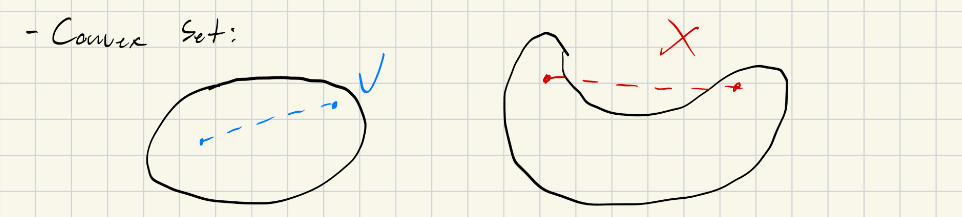
\includegraphics[width=0.9\linewidth]{l10_1.png}
\end{figure}
    \item A line connecting any two points in the set is fully contained in the set
    \item Standard examples:
    \begin{itemize}
        \item Linear Subspaces- $Ax = b$
        \item Half spaces/box/polytope- $Ax\leq b$
        \item Ellipsoids- $x^TPx\leq 1, P>0$
        \item Cones- $x_1\geq ||x_{2:N}||_2$ (Second order cone, "ice cream cone")
    \end{itemize}
    \end{itemize}
    \item Convex Function:
    \begin{itemize}
        \item A function $f(x): \mathbb{R}^n\rightarrow\mathbb{R}$ who's epigraph is a convex set
        %insert figure here
        \begin{figure}[H]
            \centering
            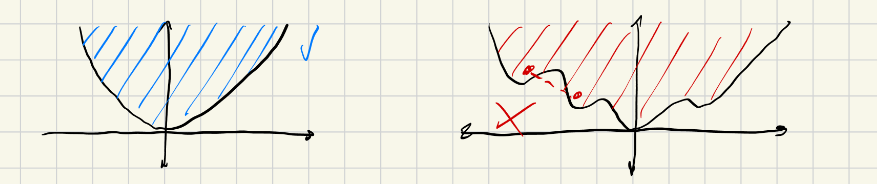
\includegraphics[width=0.9\linewidth]{l10_2.png}
        \end{figure}
        \item Epigraph is everything above the bowl
        \item Epigraph on the right is not a convex function
        \item Standard examples:
        \begin{itemize}
            \item Linear- $f(x) = c^Tx$
            \item Quadratic- $f(x) = \frac{1}{2}x^TQx + q^Tx, \quad Q\geq0$
            \item Norms- $f(x) = |x|$ (Any norm)
        \end{itemize}
    \end{itemize}
    \item Convex Optimization Problem: minimize a convex function over a convex set
    \item Standard examples:
    \begin{itemize}
        \item Linear Program (LP) : $f(x),c(x)$ both linear
        \item Quadratic Program (QP): quadratic $f(x)$, linear $c(x)$
        \item Quadratically constrained QP (QPQC): quadratic $f(x)$, ellipsoid $c(x)$
        \item Second order cone program (SOCP): linear $f(x)$, cone $c(x)$
    \end{itemize}
    \item Convex optimization problems don't have any spurious local optima that satisfy KKT conditions
    \item $\Rightarrow$ if you find a local KKT solution, you have the solution
    \item Practically, Newton's method converges really fast and reliably (5 to 10 iterations max)
    \item Can bound solution time for real-time control
\end{itemize}
\section{Convex MPC}
\begin{itemize}
    \item Think ``Constrained LQR"
    \item Remember from DP, if we have a cost-to-go function $V(x)$, we can get $u$ by solving a one-step problem:
    \begin{align*}
        u_k &= \text{arg}\min_u l(x,u) + V_{k+1}(f(x,u))
        \\
        &= \text{arg}\min_u \frac{1}{2}u^TRu + (Ax+Bu)^TP_{k+1}(Ax+Bu)
    \end{align*}
    \item We can add constraints on $u$ to this one-step problem, but this will perform poorly because $V(x)$ was computed without constraints
    \item There's no reason I can't add more steps to the one-step problem:
    \begin{align*}
        \min_{x_{1:H},u_{1:H-1}}\sum_{k+1}^{H-1}\frac{1}{2}x_k^TQx_k + \frac{1}{2}u_k^TRu_k + x_H^TP_Hx_H
    \end{align*}
    \item $H<<N$ is called ``Horizon"
    \item With no additional constraints, MPC (``Receeding horizon horizon") exactly matches LQR for any $H$
    \item Intuition: explicit constrained optimization over first $H$ steps gets the state close enough to the reference that the constraints are no longer active and LQR cost to go is valid farther into the future
    \item In general:
    \begin{itemize}
        \item A good approximation of $V(x)$ is important for good performance
        \item Better $V(x)\Rightarrow$ shorter horizon
        \item Longer $H\Rightarrow$ less reliance on $V(x)$
    \end{itemize}
\end{itemize}
\subsection{Example}
\begin{itemize}
    \item Planar Quadrotor
    %insert figure here
    \begin{figure}[H]
        \centering
        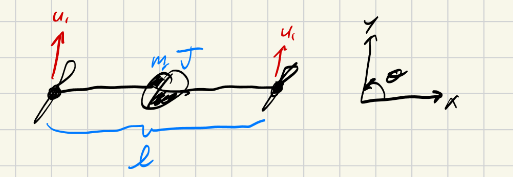
\includegraphics[width=0.6\linewidth]{l10_3.png}
    \end{figure}
    \begin{align*}
        m\ddot{x} &= -(u1 + u_2)\sin(\theta)
        \\
        m\ddot{y} &= (u_1 + u_2)\cos(\theta)
        \\
        J\ddot(\theta) &= \frac{1}{2}l(u_2-u_1)
    \end{align*}
    \item Linearize about hover:
    \begin{align*}
        \Rightarrow u_1&=u_2 = \frac{1}{2}mg
        \\
        \Delta\ddot{x} &\approx -g\Delta\theta
        \\
        \Delta\ddot{y} &\approx \frac{1}{m}(\Delta u_1 + \Delta u_2) \\
        \Delta\ddot{\theta} &\approx\frac{1}{J}\frac{l}{2}(\Delta u_2 - \Delta u_1)
        \\
        \begin{bmatrix}
            \Delta \dot{x} \\
            \Delta \dot{y} \\
            \Delta \dot{\theta}\\
            \Delta \ddot{x} \\
            \Delta \ddot{y} \\
            \Delta \ddot{\theta}
        \end{bmatrix}
        &= 
        \begin{bmatrix}
            0 & 0 & 0 & 1 & 0 & 0 \\
            0 & 0 & 0 & 0 & 1 & 0 \\
            0 & 0 & 0 & 0 & 0 & 1 \\
            0 & 0 & -g & 0 & 0 & 0 \\
            0 & 0 & 0 & 0 & 0 & 0 \\
            0 & 0 & 0 & 0 & 0 & 0 \\
        \end{bmatrix}
        \begin{bmatrix}
            \Delta x \\
            \Delta y \\
            \Delta\theta \\
            \Delta \dot{x} \\
            \Delta \dot{y} \\
            \Delta \dot{\theta}
        \end{bmatrix}
        + 
        \begin{bmatrix}
            0 & 0 \\
            0 & 0 \\
            0 & 0 \\
            0 & 0 \\
            \frac{1}{M} & \frac{1}{m} \\
            -\frac{l}{2J} & \frac{l}{2j}
        \end{bmatrix}
        \begin{bmatrix}
            \Delta u_1 \\
            \Delta u_2
        \end{bmatrix}
    \end{align*}
    \item MPC cost function
    \begin{align*}
        J &= \sum_{k=1}^{H-1}\frac{1}{2}(x_k - x_{ref})^TQ(x_k-x_{ref}) + \frac{1}{2}\Delta u_k^TR\Delta u_k + \frac{1}{2}(x_k-x_{ref})^TP_H(x_k-x_{ref})
    \end{align*}
    \item Due to linearization, the model can break of going outside the region where the linearization is valid. To deal with this, can add constraint to keep control within valid region. i.e.- keeping $\theta$ to a small enough values.
\end{itemize}

\end{document}
